%#! platex thesis.tex
\documentclass[a4paper,12pt]{jreport}
\usepackage{jgraduate}          % 卒論・修論用スタイル

%% 索引作成
%\usepackage{makeidx}
% dvipdfmxを使用しない場合はオプションを変更すること
\usepackage[dvipdfmx]{graphicx}
% 数字付きリストでラベルを使う
\usepackage{enumerate}
% 数学記号など
\usepackage{amsmath}
\usepackage{amssymb}
\usepackage{amsthm}
% URLをいい感じにする
\usepackage{url}
\usepackage{cite}

%------------------------------
% 余白設定
%------------------------------
\usepackage[left=27mm,right=27mm,top=45mm,bottom=45mm,%
 headheight=5mm,headsep=10mm,%
 footskip=12mm%
 ]{geometry}

%------------------------------
% hyperref
%  日本語の文字コード設定が分からない人はコメントアウトすること.
%------------------------------
% PDF化したときにしおりが作成され,図表へのジャンプも可能となる.
\usepackage{atbegshi}
% Mac/Linuxの場合
%   ※Ubuntuの場合はEUC-UCS2を自分で入れないとダメ.
\AtBeginShipoutFirst{\special{pdf:tounicode EUC-UCS2}}
%% Winの場合
%\AtBeginShipoutFirst{\special{pdf:tounicode 90ms-RKSJ-UCS2}}
% 以下は共通
\usepackage[dvipdfm,a4paper,bookmarks,bookmarksnumbered,%
 bookmarksopen=false,pdfstartview={FitH},%
 bookmarkstype=toc,%
 setpagesize=false,%
 pdfauthor={新堂 風},%
% setpagesize=false,% PDFのサイズがおかしい場合はこれを有効化
 pdftitle={(タイトル未定)遠隔医療システムにおける処方箋予測に向けた手書き医療用語認識に関する研究}]{hyperref}

%----------------------------------------------------------------------
% 設定
%----------------------------------------------------------------------
% 目次の深さはsubsubsectionまで
\setcounter{tocdepth}{3}

% 基準となる図の幅
\newlength\figurewidth
\setlength{\figurewidth}{0.8\textwidth}
% 縦に並べた図の間の基準となるスペース
\newlength\figuresep
\setlength{\figuresep}{0.8\floatsep}

%----------------------------------------------------------------------
% 文書基本情報
%----------------------------------------------------------------------
% タイトル
\title{未定}

% 著者
\author{新堂 風}

% 所属
% 学部
\university{九州大学}
\department{工学部}
\major{電気情報工学科}
%% 修士・博士
%\university{九州大学大学院}
%\department{システム情報科学府}
%\course{修士課程}
%\major{情報知能工学専攻}
%\submajor{知的情報システム工学コース}

% 提出日(月までを書く)
\date{令和2年2月}

%% 書いている途中では以下のようにしておくと一部だけをタイプセットできる
%\includeonly{intro}

%======================================================================
% テキスト開始
%======================================================================
\begin{document}
% 表紙
\maketitle
% 表紙はページ番号を出力しない
\thispagestyle{empty}

%----------------------------------------------------------------------
% 概要
%----------------------------------------------------------------------
\begin{abstract}
 Portable Health Clinic(以下,PHC) は発展途上国農村部における健康促進に向けた遠隔医療システムである.ヘルスアシスタントと呼ばれるスタッフが複数の健康測定器具を医者のいない農村部に持ち込み,村民に対して健康診断を行う.健康診断の結果,医者からの診断が必要であると判断された患者は都市部にいる医者と電話を通して繋がり,医者が直接診断できない発展途上国農村部においても人々は診断を受けることができる.このシステムでは,医者は患者を診断しながら症状や処方薬などをノートに取り,通話後にそれをコンピュータに入力して処方箋を作成する.このときにノートに書かれた手書き文字を認識し,その情報を元に処方箋を予測してコンピュータに入力する手間を削減できれば,医者の時間を節約でき,医者はさらに多くの人々の診断を行うことができる.

現在医療用語に特化したデータセットがオープンソースとして存在しないため,PHCにおける過去の処方箋データから頻出する単語を座標の時系列データとして収集する.様々な手書き文字に対応するため,本研究では多様な提供者から大量のデータを得る必要があるが,十分なデータ量を確保するためには非常に多くの労力と時間を要する.十分な量のデータ収集なしに高精度の文字認識ができるオンライン手書き医療用語認識の実現を目指して,現在データ拡張手法を用いたオンライン手書き医療用語認識\cite{takahashi}が開発されている.先行研究\cite{takahashi}は,ストロークの回転と平行移動によってデータ量を水増しするStroke Rotation and Parallel-shift(SRP)手法を用いている.この用語認識はデータ量が少ない状況での学習を実現でき,高精度でのオンライン手書き医療用語認識が可能であることが確認されている.しかしSRP手法において回転の大きさ,平行移動の大きさは筆者が文字の形を崩さないと判断できる範囲で設定しているため,データを高倍率で拡張した場合に同じような値を用いてしまい,拡張後に同じようなデータが増えて学習精度が低くなる原因になってしまう.そのためこの用語認識は学習の際にランダムに設定された回転の大きさと平行移動の大きさの組み合わせにより,認識精度にばらつきが出てしまうという問題がある.

本論文では,処方箋の予測に向けたシステムの初期研究として,安定して高精度で学習することができるオンライン手書き医療用語認識システムを提案する.またオンライン手書き文字のデータ拡張手法として文字の縦横比を変更しデータ量を水増しするRatio手法を新たに提案する.Ratio手法は文字の縦横比を変更するため,拡張後に文字のストロークが重なることがなく文字の形を大きく変えてしまうことがないままデータの多様化を行うことができる.本論文では既存のSRP手法とRatio手法を組み合わせてデータ拡張を実現した.収集した15991語のデータを用いて,SRP手法とRatio手法でデータ拡張を行った後にBidirectionalLSTMで学習を行った結果,480語のクラスにおいて平均精度93.0\%,最小精度92.1\%で単語を認識した.この結果はSRP手法のみの場合の認識精度と比べて平均精度は3.5\%,最小精度は14.7\%向上した.データ拡張を行わなかった場合の認識精度と比べて平均精度は19.6\%,最小精度は73.1\%向上した.
\end{abstract}
%----------------------------------------------------------------------
% 目次のページ番号は1から
\setcounter{page}{0}
% 目次
\tableofcontents

% 本文のページ番号はアラビア数字
\pagenumbering{arabic}

%======================================================================
% 本文ここから
%======================================================================

% 章ごとのファイルを読み込む
% YaTeXなら各ファイルを読み込む行でC-c gでジャンプできる

% はじめに
%#! platex thesis.tex

%======================================================================
\chapter{はじめに}
\label{cha:intro}
\section{研究背景}
\label{sec:background}
Portable Health Clinic (以下,PHC)は発展途上国農村部における,健康促進のための遠隔医療システムである\cite{ahmed15:portable}.ヘルスアシスタントと呼ばれるスタッフが複数の健康測定器具を医者のいない農村部に持ち込み,村民に対して健康診断を行う.健康診断の結果,医者からの診断が必要であると判断された患者は都市部にいる医者と電話を通して繋がり,診断を受けることができる.このシステムによって,医者が直接診断できない発展途上国農村部においても人々は診断を受けることができる.このシステムでは,医者は患者を診断しながら症状や処方薬などをノートに取り,通話後にそれをコンピュータに入力して処方箋を作成する.このときにノートに書かれた手書き文字を認識し,その情報を元に処方箋を予測してコンピュータに入力する手間を削減できれば,医者の時間を節約でき,医者はさらに多くの人々の診断を行うことができる.

\section{研究目的}
本研究の目的は,遠隔医療における,処方箋予測に向けたオンライン文字認識に適したデータの拡張方法を確立することである.オープンソースのオンライン文字認識用データセットのうち,医療用語に特化したものは存在していないため,文献\cite{takahashi}では独自にデータ収集を行っている.しかしデータの収集には多くの時間と労力を要するため,文献\cite{takahashi}ではデータ拡張を行ってデータ量を水増している.***************そのため,この用語認識は学習の際のデータのとり方により認識精度にばらつきが出てしまうという問題がある.


現在,オンライン文字認識の研究においてデータ拡張を行っているものは非常に少なく,高精度を保って学習できるオンライン文字認識の拡張方法は未だ確立されていない.機械学習においてデータ量は精度を大きく左右する重要なパラメータである.オフライン文字認識については多くのデータ拡張方法が研究されているが,オンライン文字認識についてもデータの拡張方法について議論がなされるべきである.


\section{論文構成}
本論文の構成は以下の通りである.第2章では,筆者らが目指しているオンライン手書き医療用語認識,及び本研究に至った取り組むべき課題について説明を行い,既存の対策の問題点をあげる.第3章では,問題解決に向け本研究で提案する手法について説明を行う.第4章では提案手法の実装について述べる.第5章では提案手法の評価について述べる.最後に第6章で本論文のまとめと今後の展望を述べる.


% 関連研究
%#! platex thesis.tex

%======================================================================
% 章見出し
\chapter{関連技術}
\label{cha:relate}
本章では,手書き文字認識技術として一般に用いられるオンライン文字認識とオフライン文字認識について説明する.さらに時系列データに対応した機械学習モデルである,再帰型ニューラルネットワークについて説明する.その後再帰型ニューラルネットワークを用いたオンライン文字認識の既存研究と,文字認識におけるデータ拡張に関する既存研究について述べる.
%----------------------------------------------------------------------

\section{手書き文字認識の種類}
\label{sec:rel_1}
手書き文字の認識は大きく2つに分けることができる.オフライン文字認識とオンライン文字認識である.オフライン文字認識は,文字の画像データにおいてそれぞれのピクセルが持つ情報を特徴量として文字を認識する技術であり,手書き文字は認識されるためにイメージスキャナやデジタルカメラによって読みとられる.
オンライン文字認識は手書き文字の$(x, y)$座標やスピード,筆圧などを特徴量として認識する技術で,通常,タブレットなどに書き込まれた文字が認識される.

オフライン文字認識は画像認識技術であるため,文献\cite{yuan12:offline}のような畳み込みニューラルネットワーク(Convolutional Neural Network,CNN)を用いた文字認識が多く研究されている.利用可能な画像データもインターネット上に多く存在するが,実際に認識を行う際には手書きされた文字をスキャナやデジタルカメラなどで読み取る必要があるなどのデメリットもある.

一方でオンライン文字認識はIAM On-Line Handwriting Database\cite{iam},CASIA Chinese Handwriting Database\cite{liu11:casia}などのデータセットが存在するが,オフライン文字認識に比べると利用可能なデータは少ない.しかし認識時においては,タブレットなどのデバイスに書き込まれた手書き文字のデータが直接使われるため,オフライン文字認識と比べると手間が少ない.また,オンライン文字認識は筆順・筆圧・書き込みにかかる時間などの,オフライン文字認識では使うことができない情報を用いて認識を行うことができるなどのメリットがある.

本研究では,医者の手書き文字は筆記体が多く使われ,画像での認識は難しいと考えられること,実際に使用する際にはスキャンやデジタルカメラによる撮影を行わず,リアルタイムでの認識を想定していることから,オンライン文字認識を用いて医者の手書き医療用語の認識を行う.

%----------------------------------------------------------------------
\section{再帰型ニューラルネットワーク}
再帰型ニューラルネットワーク(Recurrent Neural Network,以下RNN)とは中間層に戻り値のある,音声,動画,文章などの時系列データを扱うニューラルネットワークである.以下でRNNの構造と,再帰型ニューラルネットワークの一種であるLong Short-Term Memory(以下,LSTM)について説明する.本研究ではLSTMを用いて機械学習を行う.
\subsection{RNNの構造}
\label{ssec:rel_2}

\begin{figure}[tb]
 \begin{center}
  \resizebox{\columnwidth}{!}{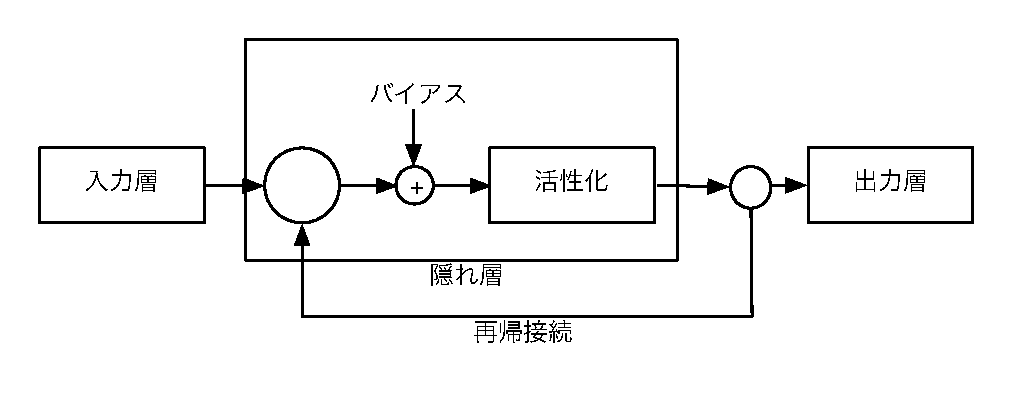
\includegraphics{img/rnn.eps}}
  \caption{RNNの構造}
  \label{rnn}
\end{center}
\end{figure}

\textbf{図~\ref{rnn}}に再帰型ニューラルネットワークの構造を示す.RNNは中間層のノードごとに戻り値があるため,現在入力されているデータより前のデータの影響を考慮して計算を行うことができる.そのためRNNは連続的な情報を入力として学習を行うことができる\cite{chakra16:bangla}.
式~\ref{eq:rnn-1}, 式~\ref{eq:rnn-2}に,RNNがそれぞれのノードにおいて行っている計算を入力値$x$と時間的順序$t$を用いて示す.
\begin{equation}
 H(t) = h(W_Hx(t) + W_{self}H(t-1) + b_H)
  \label{eq:rnn-1}
\end{equation}
\begin{equation}
 Y(t) = y(W_YH(t) + b_Y)
  \label{eq:rnn-2}
\end{equation}
ここにおいて$H(t)$は隠れ層の出力であり,$W_H$は隠れ層への入力の重み,$W_{self}$は戻り値の重み,$b_H$は隠れ層へのバイアス,$Y(t)$はネットワークの出力,$W_Y$は隠れ層の出力の重み,$b_Y$は出力へのバイアス,$y()$と$h()$はそれぞれ出力層と隠れ層の活性化関数である.式より,隠れ層の出力は隠れ層への入力$x(t)$だけでなく,隠れ層からの1つ前の出力$H(t-1)$の影響も受けていることがわかる.したがってネットワークの出力$Y(t)$は$x(t)$と$x(t-1)$の影響を受けていると言える.この計算は最初をのぞいた全ての入力において行われている.

\begin{figure}[tb]
 \begin{center}
  \resizebox{\columnwidth}{!}{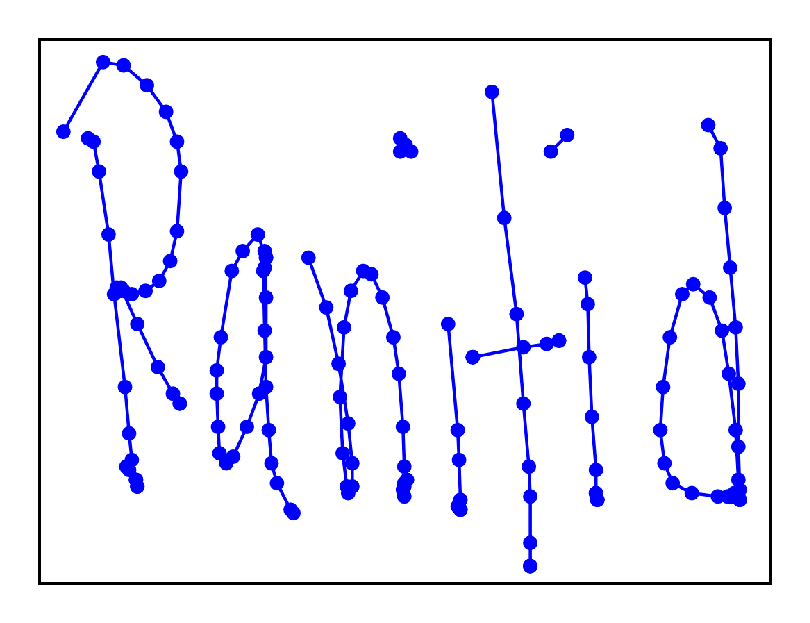
\includegraphics{img/ranitid.eps}}
  \caption{文字を点で表した図}
  \label{original}
\end{center}
\end{figure}

\textbf{図~\ref{original}}に認識する手書き文字の例を示す.このように,手書き文字は検出された座標が時間的順序に従って並んだものであると言える.オフライン文字認識では,手書き文字を画像データとして捉えるため,点の時間的順序を考慮に入れずに認識を行う.RNNの入力に連続した手書き文字の点データを用いることで,オンライン文字認識ではその時間的順序を考慮に入れて認識を行うことができる.

しかし,実際にRNNで出力に反映できる過去の入力情報は短く,時系列10ステップ分程度であると言われている\cite{okatani15:deep_learning}.

\subsection{LSTM}
\label{ssec:lstm}

\begin{figure}[tb]
 \begin{center}
  \resizebox{\columnwidth}{!}{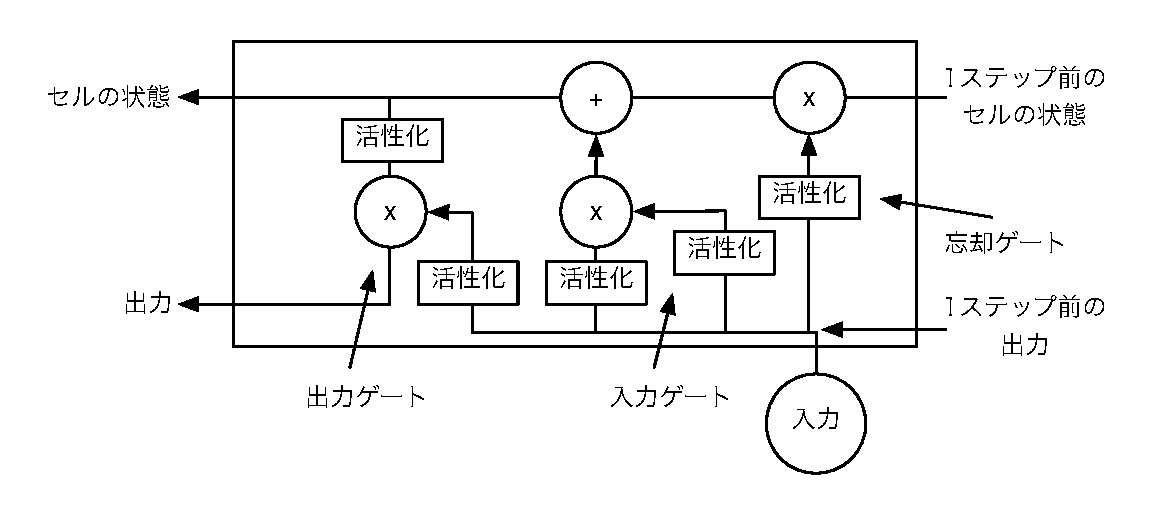
\includegraphics{img/lstm.eps}}
  \caption{LSTMブロックの構造}
  \label{lstm}
\end{center}
\end{figure}

\textbf{図~\ref{lstm}}にLSTMブロックの構造を示す.LSTMはRNNよりも長期にわたる記憶を実現するための方法のひとつで,RNNの隠れ層の各ユニットをLSTMブロックに置き換えたものである.RNNのユニットと異なり,LSTMブロックは記憶を持ったセルの構造をしている.ゲートと呼ばれる特殊な構造がセルに情報を与えるかセルの情報を除去するかを決める.

忘却ゲートがセル内の情報をリセットし,入力ゲートは,入力が現在のセルにどれだけ影響を与えるか決める.出力ゲートは出力が残りのネットワークにどれだけの影響を与えるか決める.この方法によってLSTMはより長い時系列データにおける再帰型ニューラルネットワークの利用を可能にしている.

%----------------------------------------------------------------------
\section{関連研究}
\label{sec:rel_3}
ここではLSTMを用いたオンライン文字認識の既存研究と,文字認識におけるデータ拡張に関する既存研究について述べる.

\subsection{直線データとBidirectionalLSTMを用いた中国語認識システム\cite{zhang18:drawing}}
\label{ssec:drawing}
文献\cite{zhang18:drawing}では中国語の手書き漢字の座標データの中から,直線上の点や近接する点など,取り除いても文字として成り立つ点を除去したのち直線データに変換し,BidirectionalLSTMを用いて認識を行っている.BidirectionalLSTMについては\ref{sec:m_learning}節で述べる.点の除去を行うことで入力データを簡易化し,さらに直線データへの変更を行うことで連続する点同士の関係性(点同士の距離,次の点への角度,同一字画上にあるかなど)を特徴量として抽出することができる.機械学習モデルにはBidirectionalLSTMを用いることで,入力されているより過去の座標の情報だけでなく未来の座標の情報も考慮に入れた学習を行うことができる.

\subsection{dropStroke手法を用いたデータ拡張と筆者同定システム\cite{yang15:dropstroke}}
文献\cite{yang15:dropstroke}では中国語の手書き漢字において,座標の時系列データから一部のストロークを除去する処理を複数回繰り返すことでデータ拡張を行い, CNN を用いたオフライン認識で筆者の同定を行っている.文字としては不完全なデータになるが筆者の特徴を大きく変えることにはならず,100\% に近い精度での筆者同定を可能にしている.ただし,ストロークを除去することで異なる文字・単語になってしまう可能性があるため,文字もしくは単語の認識においてこの手法は適切であるとは言えない.

同著者からは,筆者同定のためのデータ拡張として dropSegment 手法というものも提案されているが\cite{yang16:dropsegment},これも異なる文字・単語に変わってしまう可能性がある.また,この手法もオフライン認識のためのデータ拡張であるため,オンライン文字認識のためのデータ拡張手法として適切であるとは言えない.

%================================================================================================
\subsection{遠隔医療システムにおける\\処方箋予測に向けた手書き医療用語認識に関する研究\cite{takahashi}}
文献\cite{takahashi}では,処方箋の予測に向けたシステムの初期研究として,再帰型ニューラルネットワークを用いたオンライン手書き医療用語認識手法の提案を行っている.また,オンライン手書き文字のデータ拡張手法として,ストロークの回転と平行移動によってデータ量を水増しするSRP(Stroke Rotation and Parallel-shift)手法を提案している.

手書き文字データは座標の時系列データとして捉えることができる.そのデータから直線上の点と近接する点を除去して機械学習への入力を簡易化し,さらに点データを直線データに変更して特徴量の抽出を行っている.文献\cite{takahashi}ではバングラデシュでの処方箋予測に向けた実装及び評価を行うが,現在医療用語に特化したデータセットがオープンソースとして存在しない.そこで,Portable Health Clinicにおける過去の処方箋データから頻出する単語を座標の時系列データとして収集し,再帰型ニューラルネットワークの一種であるBidirectionalLSTMを用いて学習を行っている.

様々な手書き文字に対応するため,文字認識では多様な提供者から大量のデータを得る必要がある.しかし,十分なデータ量を確保するためには非常に多くの労力と時間を要する.そこで筆者らはSRP手法を提案している.

収集した15991語のデータを用いて,SRP手法でデータ拡張を行った後にBidirectionalLSTMで学習を行った結果,480語のクラスにおいて89.5\%の精度で単語を認識している.この結果はデータ拡張を行わなかった場合の認識精度と比べて16.1\%高かい.
しかし,SRP手法において回転の度合い,平行移動の度合いは筆者が文字のパラメーターを崩さないと判断できる範囲で設定しており,データを高倍率で拡張した場合,同じようなデータが増えてしまい学習精度が低くなる原因になる.そのため,この用語認識は学習の際のデータのとり方により認識精度にばらつきが出てしまうという問題がある.
% 以下はRefTeX用
%%% Local Variables:
%%% mode: yatex
%%% TeX-master: "thesis"
%%% End:


%提案手法
%#! platex thesis.tex

%======================================================================
\chapter{LSTMを用いた手書き医療用語認識とSRP手法及びRatio手法によるデータ拡張}
\label{cha:propose}
本章では,先行研究のBidirectionalLSTMを用いたオンライン手書き医療用語認識を説明する.また,オンライン文字認識用のデータ拡張手法として先行研究のSRP手法を説明し,新手法としてRatio手法を提案する.
%----------------------------------------------------------------------
\section{システムの概要}
\label{sec:concept}
\textbf{図~\ref{sys_concept}} にシステムの概要を示す.提案システムでは,タブレットから収集した手書き医療用語の座標データに対して前処理を行う.その後学習プロセスでは前処理後のデータにSRP手法を用いたデータ拡張を適用し,機械学習における学習データとする.推定プロセスでは,学習を行ったモデルに前処理後のデータを入力し,用語を推定する.

ニューラルネットワーク構造とデータ前処理,特徴量抽出に関しては\ref{ssec:drawing}項の文献\cite{zhang18:drawing}を参考にする.以下,各手順について述べる.

\begin{figure}[tb]
 \begin{center}
  \resizebox{\columnwidth}{!}{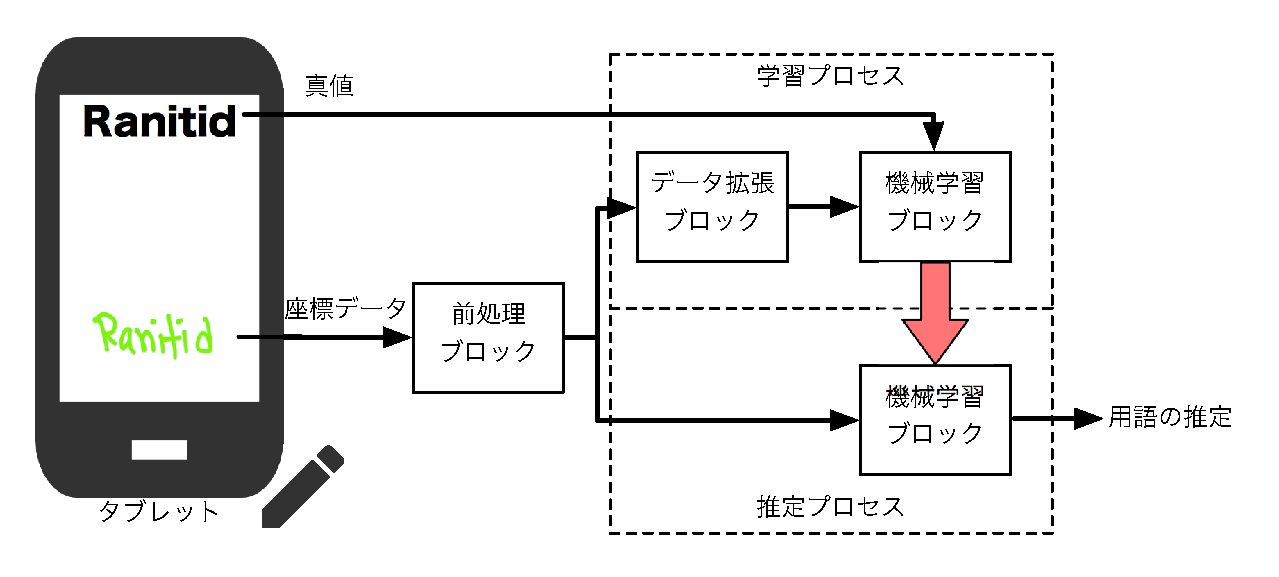
\includegraphics{img/system_structure.eps}}
  \caption{提案システムの概要}
  \label{sys_concept}
\end{center}
\end{figure}

\section{前処理ブロック}
\label{preprocess}
\textbf{図~\ref{preprocess}} に前処理ブロックの概要を示す.前処理ブロックでは,点の除去,正規化,特徴量抽出を行う.直線上の点や近接する点といった,取り除いても文字として成り立つような点の除去を行い,その後正規化を行う.特徴量抽出では点データを直線データへ変換する.以下,前処理ブロックにおける各処理を示す.

\begin{figure}[tb]
 \begin{center}
  \resizebox{\columnwidth}{!}{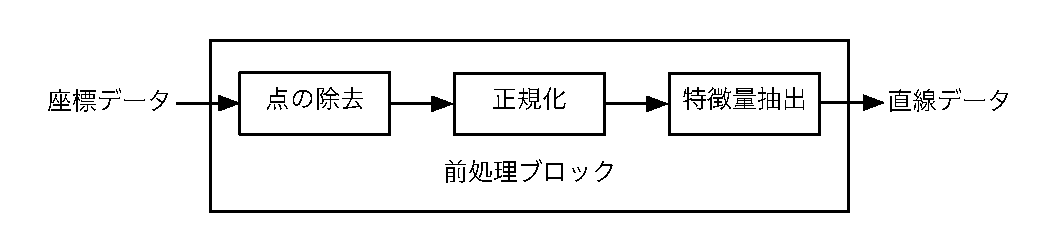
\includegraphics{img/preprocess.eps}}
  \caption{前処理ブロックの概要}
  \label{preprocess}
\end{center}
\end{figure}

\subsection{点の除去}
\label{remove_points}
この処理では,各単語におけるデータの提供者ごとの点の数の差を小さくするため,取り除いても文字として成り立つような点の除去を行う.本研究では直線上の点と近接する点の2種類を除去する.

収穫する医療用語手書きデータは,\textbf{図~\ref{original}}で示したように$(x, y)$座標の時系列データとして存在している.本研究では文献\cite{zhang18:drawing}に従って,これに各点の筆順情報$s$を合わせた$(x, y, s)$を収集する.1つの単語を式~\ref{dataSt}のように収集する.
\begin{equation}
 [[x_1, y_1, s_1], [x_2, y_2, s_2],..., [x_n, y_n, s_n]]
 \label{dataSt}
\end{equation}
$x_i$と$y_i$は点の座標,$s_i$はその点が何画目のストローク上にあるかを示したものである.

手書きデータは書くスピードの違いなどが原因で,同じ単語でもデータ提供者によって点の数が大きく異なってしまい,うまく認識ができない可能性がある.取り除いても文字として成り立つような点の除去を行うことでデータ提供者ごとの点の数の差を小さくすることができる.

本研究で除去する点は2種類ある.1つ目は直線上の点である.\textbf{図~\ref{extra}(a)}に除去する点のイメージ図を示す.点$i$が点$i-1$と点$i+1$の直線上にある場合,点$i-1$から点$i$を通って点$i+1$に向かう線は$i$を除去しても直線として成り立つため,$i$を除去する.$\Delta{x_i}=x_{i+1}-x_i$,$\Delta{y_i}=y_{i+1}-y_i$として式~\ref{eq:cos}を用いてコサインの値を算出し,その値が閾値$T_{cos}$より大きい場合,点$i$を除去する.
\begin{equation}
 \frac{\Delta{x_{i-1}}\Delta{x_i}+\Delta{y_{i-1}}\Delta{y_i}}
 {{(\Delta{x^2_{i-1}}+\Delta{y^2_{i-1}})}^{0.5} {(\Delta{x^2_i}+\Delta{y^2_i})}^{0.5}}
 >T_{cos}
  \label{eq:cos}
\end{equation}
\textbf{図~\ref{extra}(b)}にオリジナルの単語データの例と, \textbf{図~\ref{extra}(c)} に直線上の点が除去された後の単語データの例を示す.

2つ目は近接する点の除去である.\textbf{図~\ref{extra}(a)}にイメージ図を示す.点$i$が点$i-1$と極端に近接している場合,点$i-1$から点$i$を通って$i+1$に向かう線は点$i-1$から点$i+1$までの直線と概ね等しくなるため,点$i$を除去する.直線上の点の除去を行った後,式~\ref{eq:dist}を用いて2点間の距離を算出し,その距離が閾値$T_{dist}$より小さい場合,点$i$を除去する.

\begin{equation}
 \sqrt{(x_i-x_{i-1})^2 + (y_i-y_{i-1})^2} < T_{dist}
  \label{eq:dist}
\end{equation}
\textbf{図~\ref{extra}(d)} に近接する点が除去された後の単語データの例を示す.

\begin{figure}[tb]
 \centering
  \begin{tabular}{c}
    \begin{minipage}[b]{0.5\hsize}
     \centering
     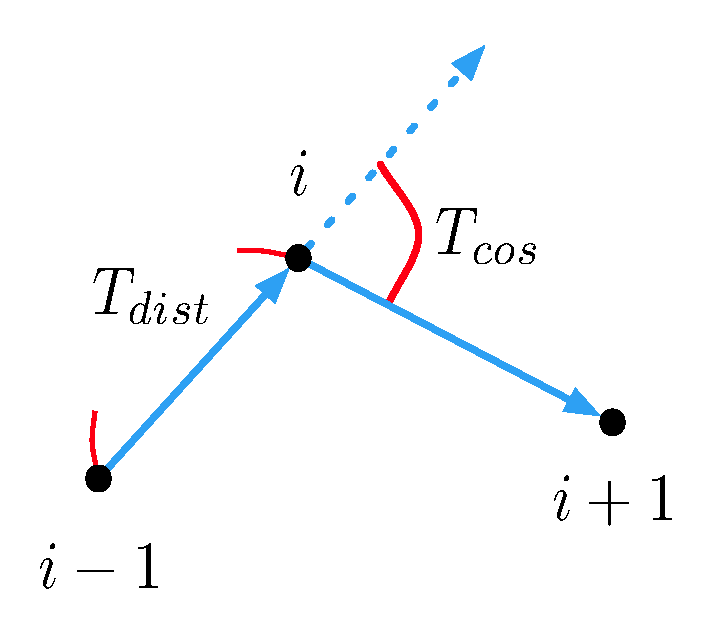
\includegraphics[keepaspectratio,scale=0.5]{img/extraPoint.eps}\\
     (a)イメージ図
    \end{minipage}
   \begin{minipage}[b]{0.5\hsize}
    \centering
    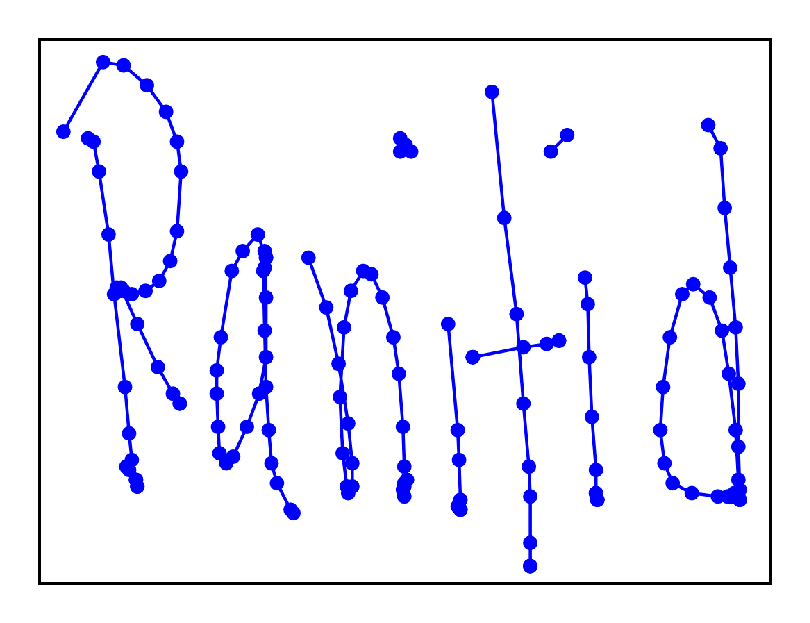
\includegraphics[keepaspectratio,scale=0.5]{img/ranitid.eps}\\
    (b)オリジナルデータ
   \end{minipage}\\
    % \hfill
   \begin{minipage}[b]{0.5\hsize}
    \centering
    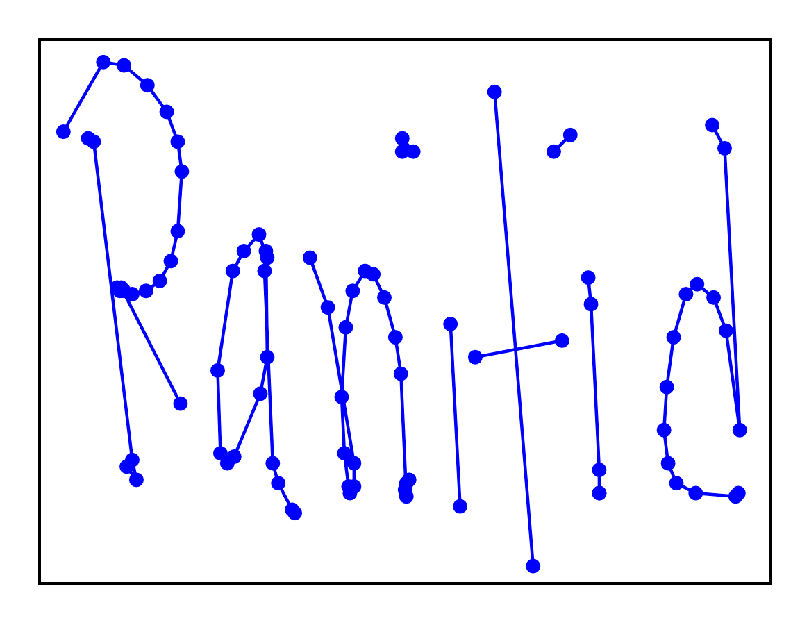
\includegraphics[keepaspectratio,scale=0.5]{img/ranitidStraight.eps}\\
    (c)直線上の点除去後
   \end{minipage}
   \begin{minipage}[b]{0.5\hsize}
    \centering
    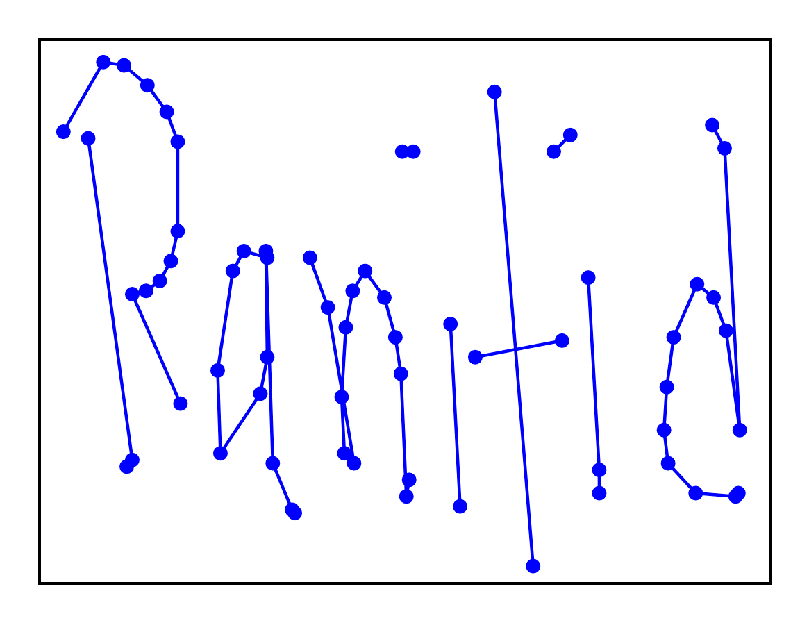
\includegraphics[keepaspectratio,scale=0.5]{img/ranitidClose.eps}\\
    (d)近接する点除去後
   \end{minipage}
  \end{tabular}
 \caption{データ前処理:余分な点の除去}
 \label{extra}
\end{figure}

\subsection{正規化}
\label{normal}
入力データをさらに簡潔にするため,点の除去を施したデータの正規化を行う.
$x$座標について説明する.全てのデータの中から最大値$x_{max}$と最小値$x_{min}$を取り出し,式~\ref{eq:normalize}を用いてある点の$x$座標$X$を$X_{nor}$に正規化する.

\begin{equation}
  X_{nor} = \frac{X - x_{min}}{x_{max}-x_{min}}
  \label{eq:normalize}
\end{equation}
$y$座標に対しても同様の計算を行い,結果的に$(x, y)$をそれぞれ$0$以上$1$以下のデータとする.

\subsection{特徴量抽出}
\label{extract}
機械学習への入力のため,特徴量を抽出する.正規化した点データ2点間を繋ぎ,直線データを作成する.直線データに変換することで,点の座標だけでなく直線の長さ,角度などより多くの特徴量を抽出することができる.線データ$L_i$は,点$i$と点$i+1$から式~\ref{eq:line}のように構成され,本研究ではこのデータを学習における入力データとする.

\begin{equation}
  L_i = [x_i, y_i, \Delta{x_i}, \Delta{y_i}, I(s_i=s_{i+1}), I(s_i \neq s_{i+1})]
  \label{eq:line}
\end{equation}
ここで,$\Delta{x_i}=x_{i+1}-x_i$,$\Delta{y_i}=y_{i+1}-y_i$であり,$I()$は括弧内の条件が真であるときに$1$でありそれ以外では$0$である.

$L_i$において$x_i$と$y_i$は直線の始点を表し,$\Delta{x_i}$と$\Delta{y_i}$は線の始点から終点までの$x$軸方向,$y$軸方向の距離を表す.また$I(s_i=s_{i+1})=1$は,直線の始点と終点が同一ストローク上にあることを示し,$I(s_i \neq s_{i+1})=1$はその直線で次のストロークに移ったことを示す.

\section{データ拡張ブロック}
\label{augment}
様々な手書き文字に対応するため,本研究では多様な提供者から大量のデータを得る必要がある.しかし,十分なデータ量を確保するためには非常に多くの労力と時間を要する.そこで,はじめに先行研究のSRP(Stroke Rotation and Parallel-shift)手法を説明する.その後,文字の縦横比を変更する変更するRatio手法を提案する.これらの手法を用いてデータ拡張を行うことで,手書き文字データの多様性を高める.

\subsection{ストロークの回転}
ストロークの始点と終点の座標から中点を求め,その点を中心にストローク上の点をそれぞれ回転させることでストローク全体を回転させる.この処理を1つのデータに対して複数回施すことで,データ拡張を行う.

\textbf{図~\ref{rotate}(a)}にストロークの回転の原理を示す.ストロークの始点を$(x_f, y_f)$,終点を$(x_l, y_l)$とする.始点と終点の中点を$(a, b)$とすると,式~\ref{eq:center}より$(a, b)$の値が求められる.

\begin{equation}
  (a, b) = (\frac{x_f+x_l}{2}, \frac{y_f+y_l}{2})
  \label{eq:center}
\end{equation}
ストローク上の任意の点の座標を$(x, y)$としたとき,その点を,点$(a, b)$を中心に角$\theta$だけ移動させた後の座標$(X, Y)$は 式~\ref{eq:rotate}で表される.

\begin{equation}
  \left(
    \begin{array}{r}
        X-a \\
        Y-b
    \end{array}
    \right)
 = \left(
  \begin{array}{rr}
      cos\theta & -sin\theta \\
      sin\theta & cos\theta
  \end{array}
  \right)
  \left(
    \begin{array}{r}
        x-a \\
        y-b
    \end{array}
    \right)
  \label{eq:rotate}
\end{equation}
\\

この式をストローク上のすべての点に用いることで,ストローク自体を角$\theta$回転させる.\textbf{図~\ref{rotate}(b)}にストローク回転前の単語データの例,\textbf{図~\ref{rotate}(c)}にストローク回転後の単語データの例を示す.この処理を,ストロークごとに角度を変えながら行うことで元のデータとは異なる形の文字・単語を生成する.それを1つの単語データに対して$N$回行い,データ量を$N$倍に拡張する.

\begin{figure}[tb]
 \centering
  \begin{tabular}{c}
   \begin{minipage}[b]{0.7\hsize}
    \centering
    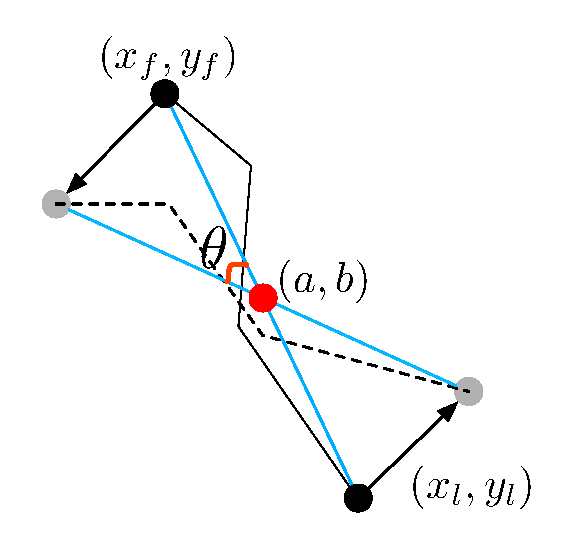
\includegraphics[keepaspectratio,scale=0.7]{img/rotate.eps}\\
    (a)回転の原理
   \end{minipage}\\
    \hfill
   \begin{minipage}[b]{0.5\hsize}
    \centering
    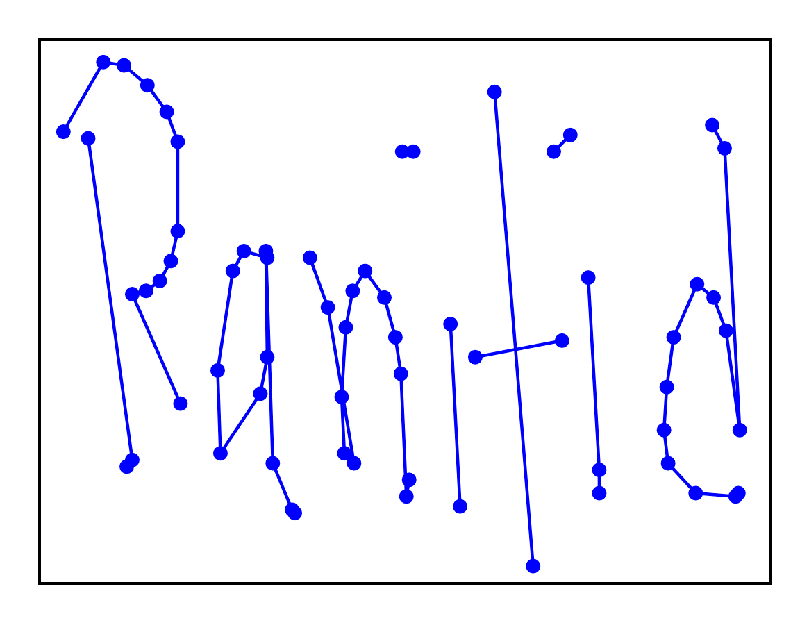
\includegraphics[keepaspectratio,scale=0.5]{img/ranitidCloseBlue.eps}\\
    (b)データ前処理後
   \end{minipage}
   \begin{minipage}[b]{0.5\hsize}
    \centering
    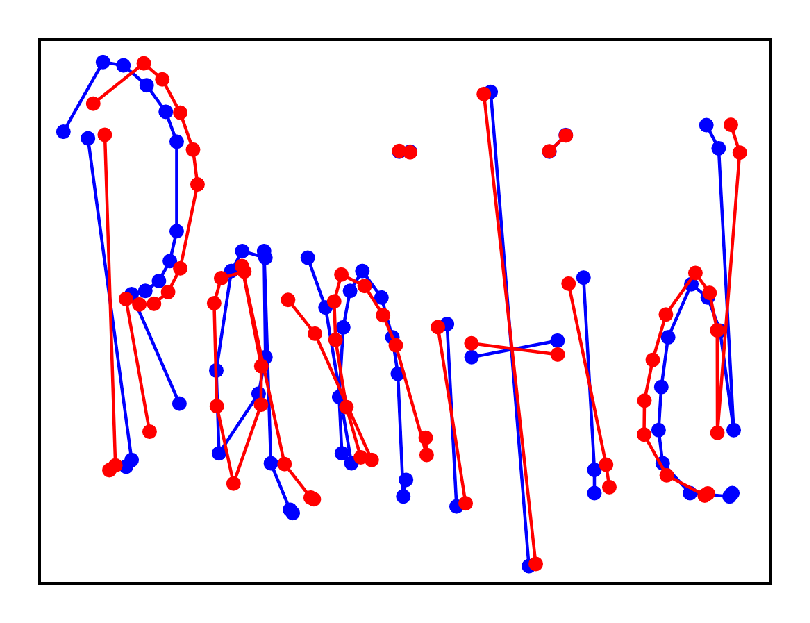
\includegraphics[keepaspectratio,scale=0.5]{img/ranitidRotateRedBlue.eps}\\
    (c)回転前(青)と回転後(赤)
   \end{minipage}
  \end{tabular}
 \caption{ストロークの回転}
 \label{rotate}
\end{figure}

\subsection{ストロークの平行移動}
ストローク上の点の座標それぞれに一定の値を加え,ストローク全体を平行移動させることでデータ拡張を行う.\textbf{図~\ref{parallel}(a)}にストロークの平行移動の原理を示す.ストローク上の任意の点の座標を$(x, y)$としたとき,その点を$x$方向に$dx$,$y$方向に$dy$だけ平行移動させた後の座標$(X, Y)$は 式~\ref{eq:parallel}で表される.

\begin{equation}
  (X, Y) = (x+dx, y+dy)
  \label{eq:parallel}
\end{equation}
この式をストローク上のすべての点に用いることで,ストローク自体を$x$方向に$dx$,$y$方向に$dy$平行移動させる.\textbf{図~\ref{parallel}(b)}にストローク平行移動前の単語データの例,\textbf{図~\ref{parallel}(c)}にストローク平行移動後の単語データの例を示す.この処理を,ストロークごとに$dx$と$dy$の値を変えながら行うことで元のデータとは異なる形の文字・単語を生成する.それを1つの単語データに対して$N$回行い,データ量を$N$倍に拡張する.

\begin{figure}[tb]
 \centering
  \begin{tabular}{c}
   \begin{minipage}[b]{0.7\hsize}
    \centering
    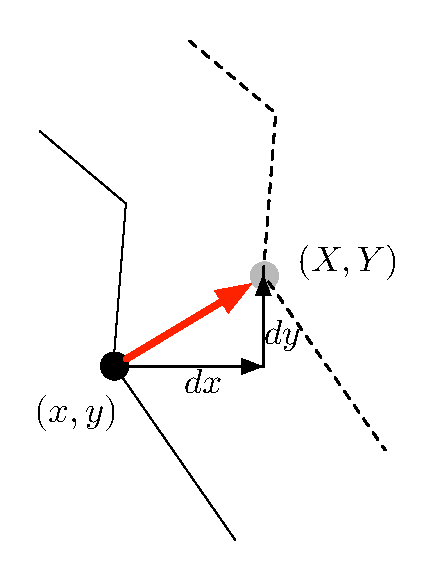
\includegraphics[keepaspectratio,scale=0.7]{img/parallel.eps}\\
    (a)平行移動の原理
   \end{minipage}\\
    \hfill
   \begin{minipage}[b]{0.5\hsize}
    \centering
    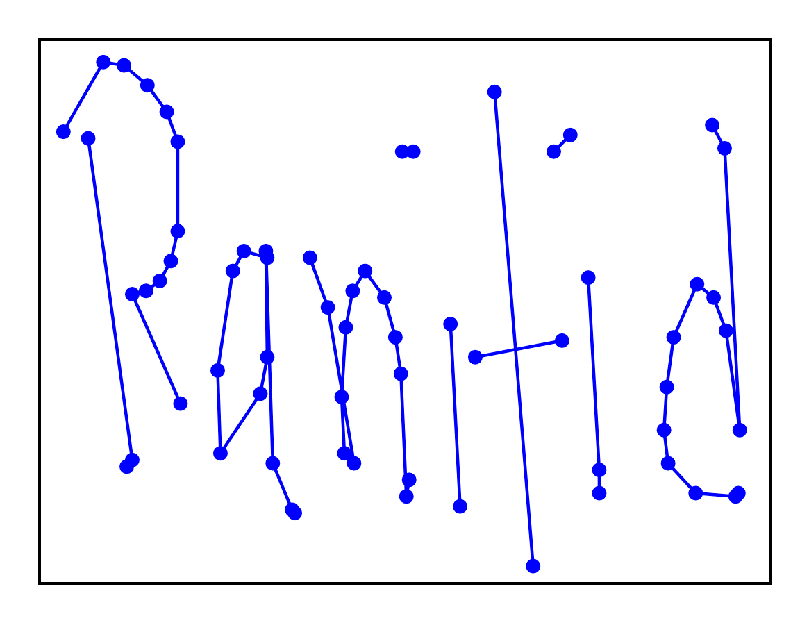
\includegraphics[keepaspectratio,scale=0.5]{img/ranitidCloseBlue.eps}\\
    (b)データ前処理後
   \end{minipage}
   \begin{minipage}[b]{0.5\hsize}
    \centering
    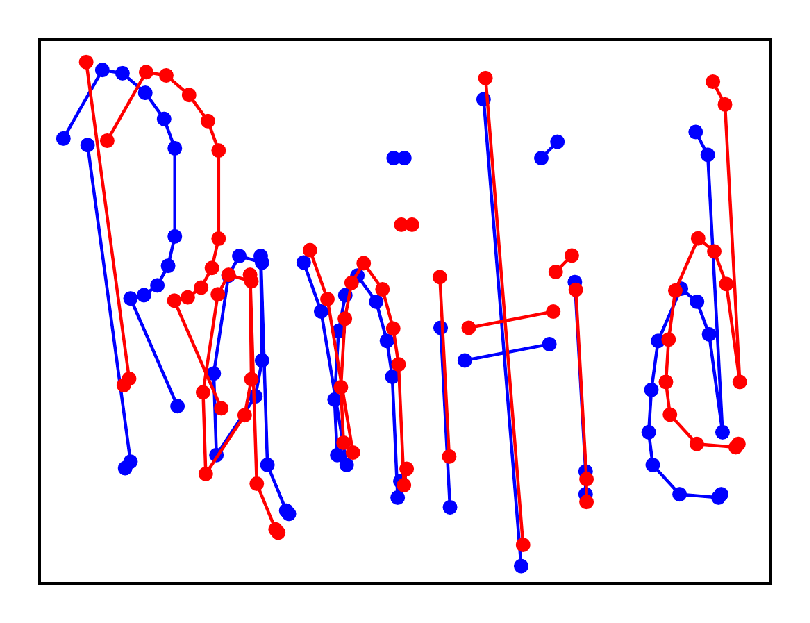
\includegraphics[keepaspectratio,scale=0.5]{img/ranitidParallelRedBlue.eps}\\
    (c)平行移動前(青)と平行移動後(赤)
   \end{minipage}
  \end{tabular}
 \caption{ストロークの平行移動}
 \label{parallel}
\end{figure}




\subsection{文字の縦横比変更}
(まだ全然かけてない,なんとなくで書いておこう)
1つの単語における,すべての点のy座標(もしくはx座標)の平均値を取り,すべての点のy座標(もしくはx座標)に対し(ここになんか書くぞ).\textbf{図}に文字の縦横比変更の原理を示す.
文字の拡張比率を$a$,1つの単語上のすべての点の$y$座標の平均を$\bar{y}$とし,同単語上の任意の点の座標を$(x, y)$としたとき,
その点の$y$座標が$\bar{y}$より大きいときに$y$方向にーーーーーー移動させた後の座標$(X, Y)$は 式~\ref{eq:yratio}で表される.

\begin{equation}
  (X, Y) = (x×1, y×(1+a))
  \label{eq:yratio}
\end{equation}
この式を単語上のすべての点に用いることで,単語全体の点をーーーーーーに移動させる.


.\textbf{図~\ref{yratio}(b)}にストローク平行移動前の単語データの例,\textbf{図~\ref{yratio}(c)}に文字の縦横比率変更後の単語データの例を示す.この処理を,拡張回数ごとに$a$と$x,y$どちらに適応するかをランダムに変えながら行うことで元のデータとは異なる形の文字・単語を生成する.それを1つの単語データに対して$N$回行い,データ量を$N$倍に拡張する.

\begin{figure}[tb]
 \centering
  \begin{tabular}{c}
   \begin{minipage}[b]{0.7\hsize}
    \centering
    %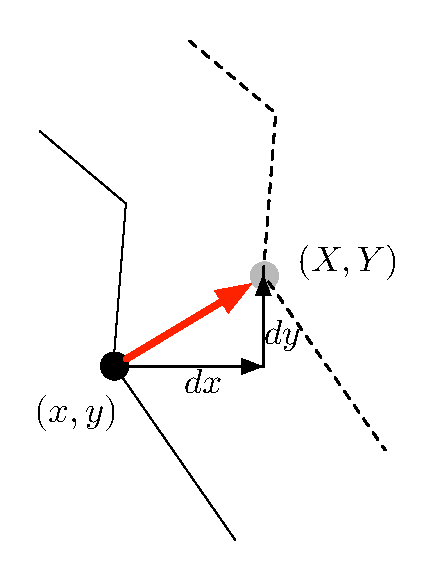
\includegraphics[keepaspectratio,scale=0.7]{img/parallel.eps}\\
    (a)平行移動の原理
   \end{minipage}\\
    \hfill
   \begin{minipage}[b]{0.5\hsize}
    \centering
    %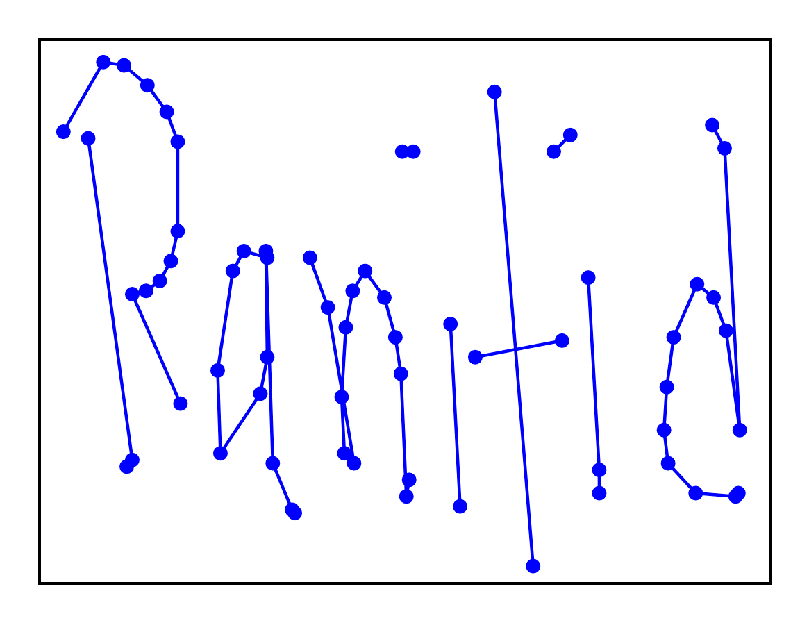
\includegraphics[keepaspectratio,scale=0.5]{img/ranitidCloseBlue.eps}\\
    (b)データ前処理後
   \end{minipage}
   \begin{minipage}[b]{0.5\hsize}
    \centering
    %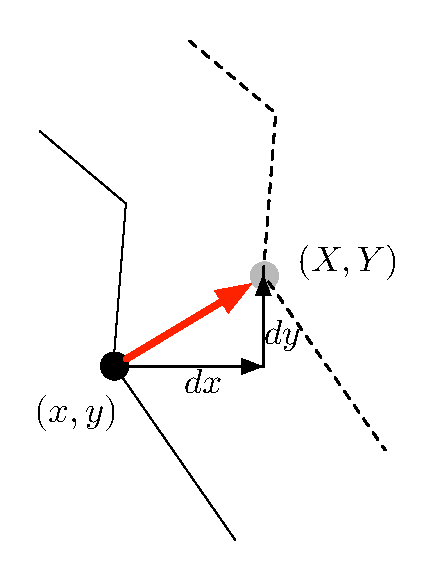
\includegraphics[keepaspectratio,scale=0.5]{img/parallel.eps}\\
    (c)ー移動前(青)とー移動後(赤)
   \end{minipage}
  \end{tabular}
 \caption{ストロークの平行移動}
 \label{yratio}
\end{figure}


\section{機械学習ブロック}
\label{sec:m_learning}
本研究ではBidirectionalLSTMを用いて学習を行う.\textbf{図~\ref{blstm}}にBidirectionalLSTMの概要を示す.BidirectionalLSTMは従来のLSTMに未来の入力から計算を行う逆方向のモデルを加え,出力を同一の出力層に統合するものである.

学習プロセスでは,データ拡張が施された直線データを入力として用いる.本研究においてBidirectionalLSTMは,現在入力されている直線データより前に書かれた直線データだけでなく,後に書かれる直線データも用いて学習を行う.

推定プロセスでは,学習が行われたモデルに前処理後のデータを入力し,用語の推定を行う.

\begin{figure}[tb]
 \begin{center}
  \resizebox{\columnwidth}{!}{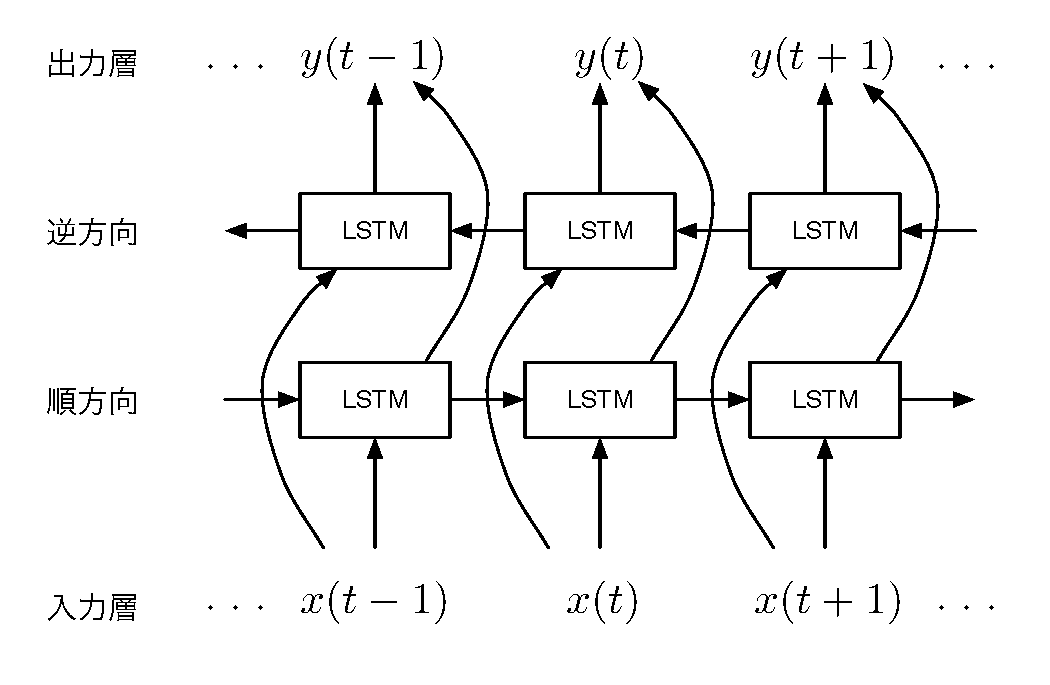
\includegraphics{img/blstm.eps}}
  \caption{BidirectionalLSTMの概要}
  \label{blstm}
\end{center}
\end{figure}

% 以下はRefTeX用
%%% Local Variables:
%%% mode: yatex
%%% TeX-master: "thesis"
%%% End:


% 実装
%#! platex thesis.tex

%======================================================================
\chapter{実装}
\label{cha:imple}
本章ではデータ収集の方法について説明し,SRP手法とLSTMを用いたオンライン手書き医療用語認識手法の実装について説明する.
%----------------------------------------------------------------------
\section{データ収集}
\label{sec:collection}
本研究では,学習に使用したいデータがオープンソースで存在していないため,既存研究において独自に収集しているデータを用いる.以下収集したデータの内容,収集手順を説明する.

\begin{figure}[tb]
 \begin{center}
  \resizebox{\columnwidth}{!}{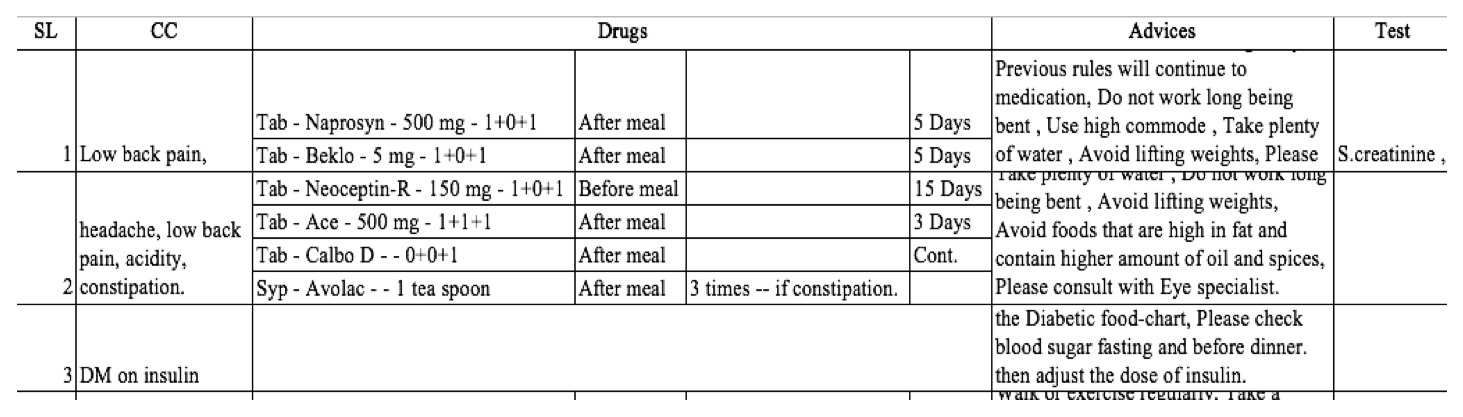
\includegraphics{img/corpus.eps}}
  \caption{PHCの処方箋データ(一部)}
  \label{corpus}
\end{center}
\end{figure}

\begin{figure}[tb]
  \begin{center}
     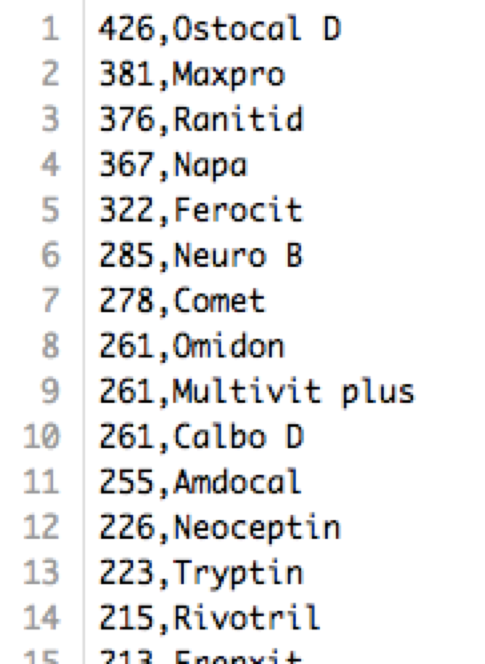
\includegraphics[keepaspectratio,scale=0.5]{img/corpus_example.png}\\
  \end{center}
 \caption{薬名欄のコーパス(一部)}
 \label{corpus_example}
\end{figure}

\subsection{医療用語コーパス}
\label{ssec:corpus}
過去の処方箋データから医療用語コーパスを作成した.コーパスとは,言語を分析するための基礎資料として書き言葉や話し言葉の資料を収集し,研究用の情報を付与したものである.本研究では医療用語の手書き認識を行う.そこで \ref{sec:background}節で述べたPHCの過去の処方箋データからコーパスを作成し,それを機械学習の正解データとして用いた. \textbf{図~\ref{corpus}}にコーパス作成に使用したPHCの過去の処方箋データを示す.8324名分の過去の処方箋データは,それぞれの欄が症状,薬名などに分けられる.\textbf{図~\ref{corpus_example}}に本研究で作成したコーパスの例として,薬名欄のコーパスの一部を示す.それぞれの欄において全ての文を1単語ごとに区切り,単語の出現回数を数えて単語を並び替えた.

本研究では薬名欄に頻出する単語(360語,英語)と医者からのアドバイス欄に頻出する単語(120語,バングラ語)を用いてコーパスを作成し,データ収集を行った.

\begin{figure}[tb]
 \begin{center}
  \resizebox{\columnwidth}{!}{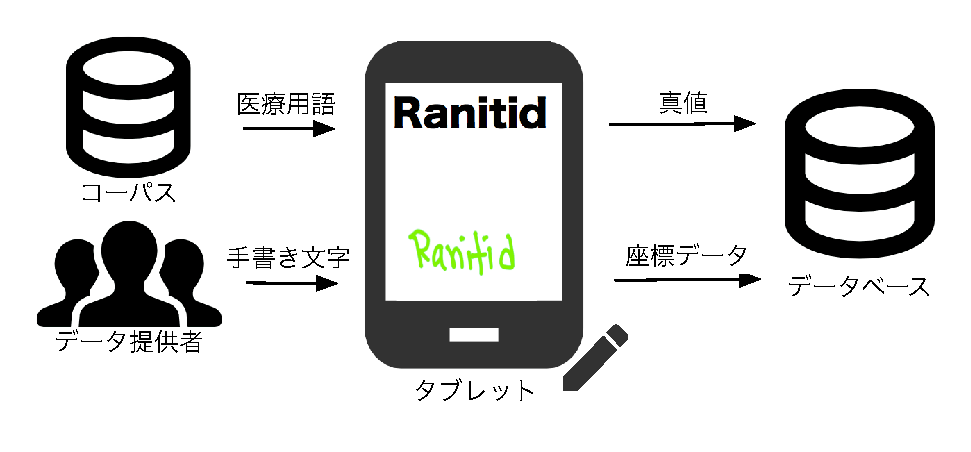
\includegraphics{img/app_structure.eps}}
  \caption{データ収集アプリの構造}
  \label{app_structure}
\end{center}
\end{figure}
%
%----------------------------------------------------------------------
\subsection{データ収集用アプリ}
\label{ssec:app}
\textbf{図~\ref{app_structure}} にデータ収集用アプリの構造を示す.オンライン手書き文字を収集するため,株式会社CodeNext\cite{codenext}にAndroidアプリの作成を依頼した.このアプリは\ref{ssec:corpus}項で作成したコーパスから単語を1語ずつ表示し,データ提供者は表示された単語をタブレットに手書きで記入する.手書きされた文字は正解データとともにデータベースに保存される.\textbf{図~\ref{app_image}}にアプリ画面のイメージ図を示す.

\begin{figure}[tb]
 \begin{center}
  \resizebox{\columnwidth}{!}{\includegraphics{img/app_image.eps}}
  \caption{データ収集アプリイメージ図}
  \label{app_image}
\end{center}
\end{figure}

\section{使用機器}
\label{sec:machine}
\textbf{図~\ref{equipments}}に使用機器を示す.データ収集用のタブレットは Samsung 社の Galaxy Tab S3 を用いた.1つのタブレットに1つのスタイラスペンが付属している.機械学習には NVIDIA社の GeForce 1080 が1枚搭載された デスクトップ PC を用いた.\textbf{~\tablename~\ref{tab:spec}}に実装環境を示す.

\begin{figure}[tb]
 \begin{center}
  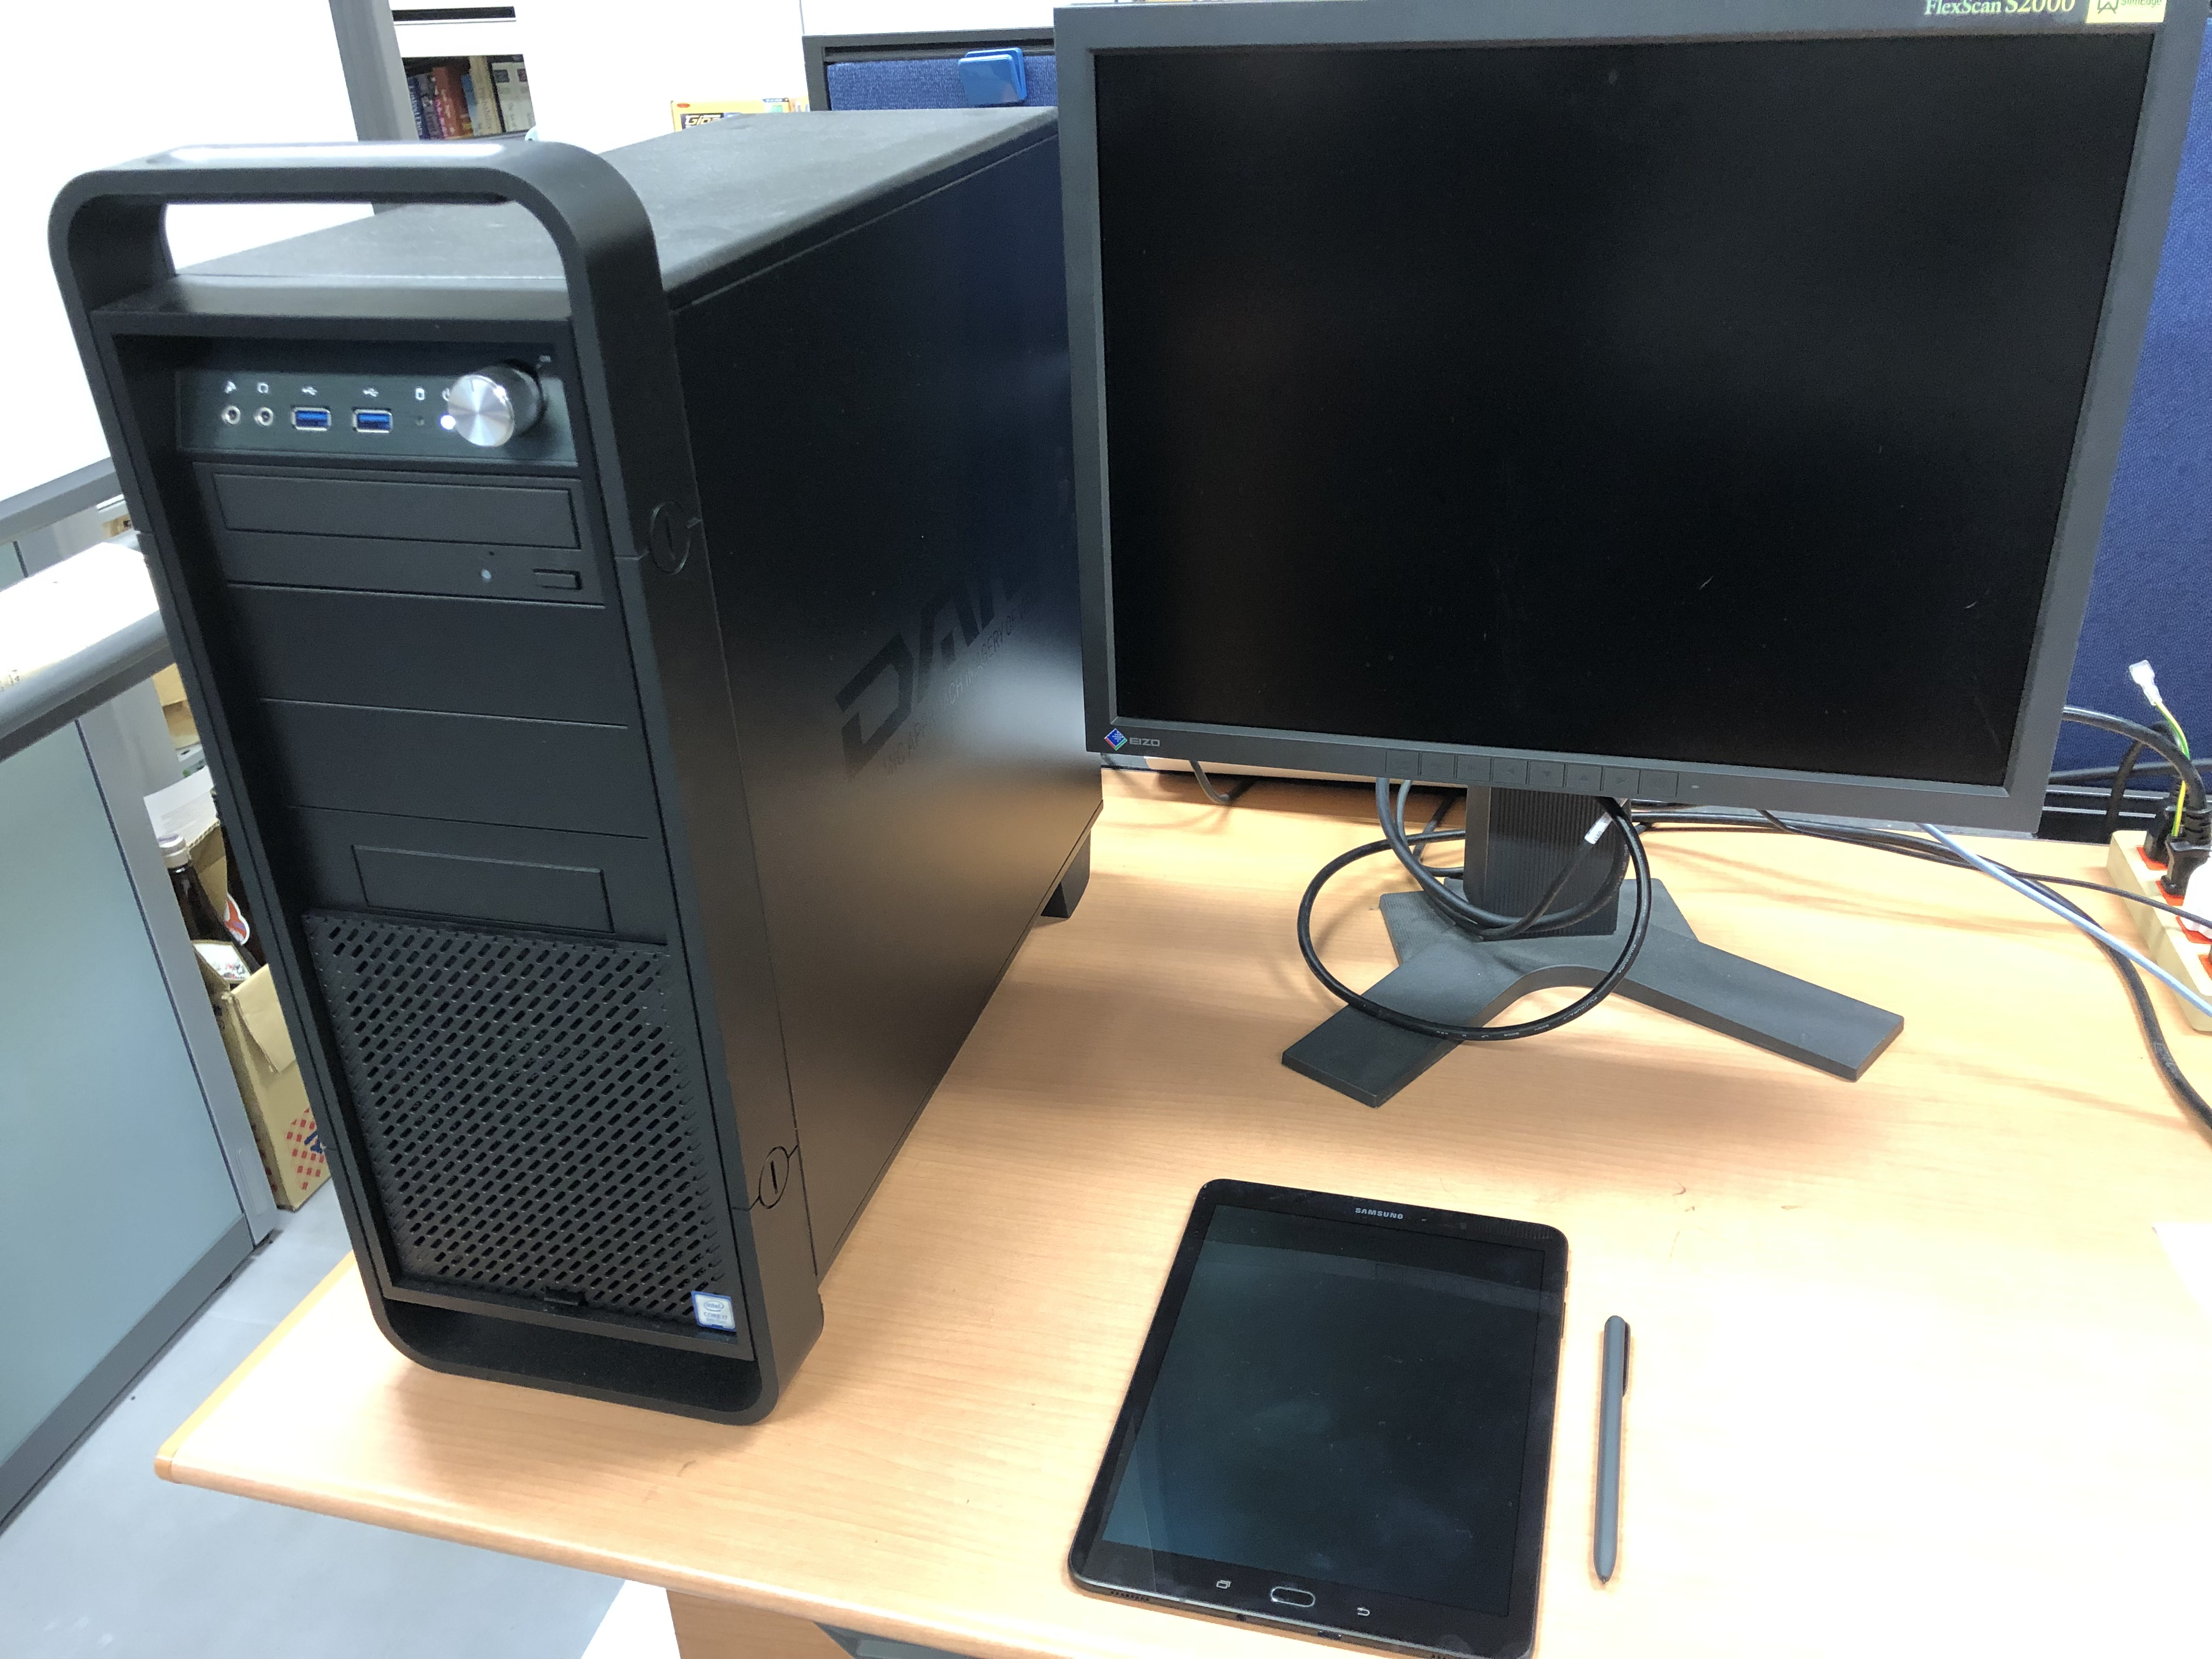
\includegraphics[keepaspectratio, scale=0.1]{img/equipments.png}
  \caption{使用機器}
  \label{equipments}
\end{center}
\end{figure}

\begin{table}[bt]
 \centering
 \caption{実装環境}
 \label{tab:spec}
 \begin{tabular}{ll}\Hline
  OS & \texttt{Ubuntu 16.04}\\
  GPU & \texttt{NVIDIA GeForce 1080}\\
  メモリ & \texttt{8GB}\\
  プロセッサ & \texttt{3.70GHz Intel Core i7-8000K}\\
  \hline
  タブレット & \texttt{Samsung Galaxy Tab S3}\\
 \Hline
 \end{tabular}
\end{table}

\section{学習モデル構造}
\textbf{図~\ref{layers}}に本研究で用いた学習モデルの構造を示す.文献\cite{zhang18:drawing}を参考に作成し,実装にはpythonのニューラルネットワークライブラリであるKeras\cite{keras}を用いた.本研究で用いるデータはデータ長が一定ではないため,データの後ろを$0$でパディングすることでデータ長最大の値である$260$に揃え,学習の入力とした.LSTM層の出力次元数は$300$に設定し,プールサイズの値の平均値をそれぞれ出力するプーリング層を配置した.その後パラメータの数を増やすために全結合層を配置した.なお,過学習を防ぐためプーリング層と全結合層の間にドロップアウト\cite{dropout}をそれぞれ$0.3$の割合で設定した.

\begin{figure}[tb]
 \centering
  \begin{tabular}{c}
    \begin{minipage}[b]{0.7\hsize}
     \centering
     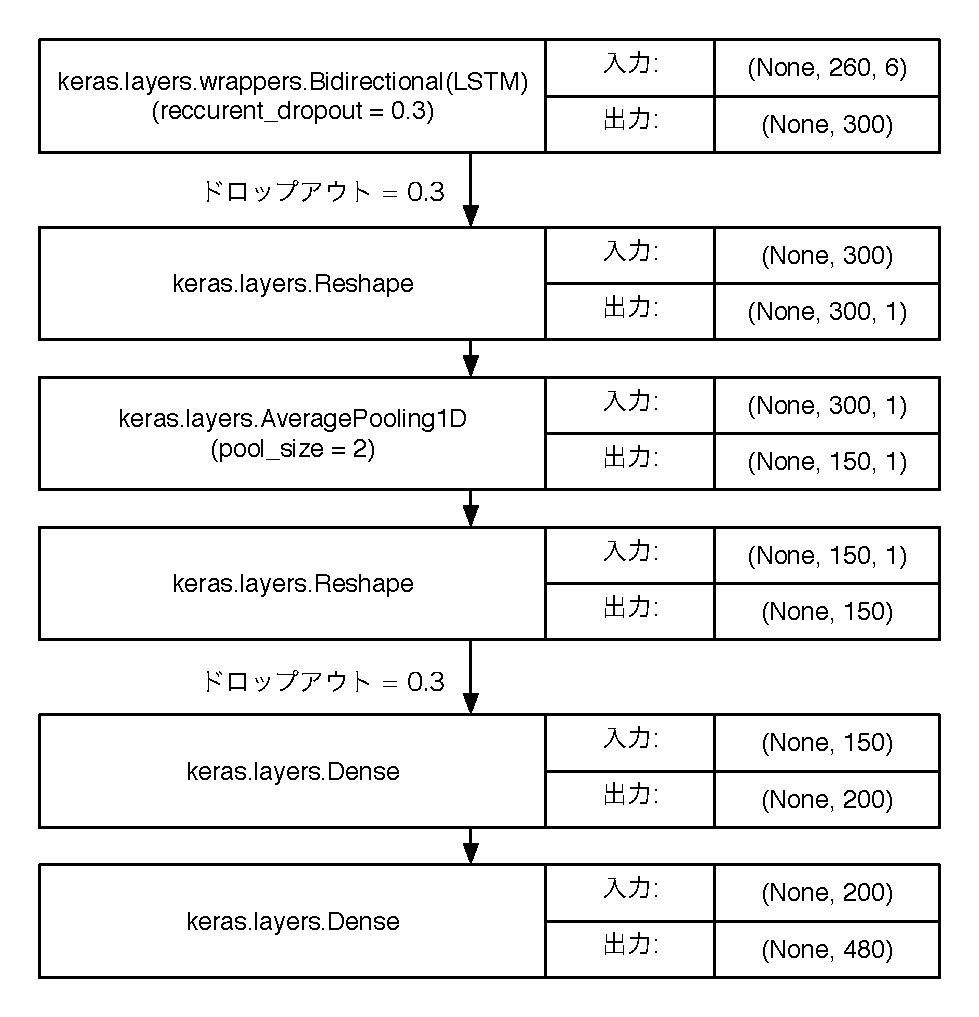
\includegraphics[keepaspectratio,scale=0.7]{img/layers.eps}\\
    \end{minipage}
  \end{tabular}
 \caption{層の構成}
 \label{layers}
\end{figure}

% 以下はRefTeX用
%%% Local Variables:
%%% mode: yatex
%%% TeX-master: "thesis"
%%% End:


% 評価
%#! platex thesis.tex

%======================================================================
\chapter{評価}
\label{cha:eval}
→→→→→→ここでおおきく評価方法を変更する

本章では,\ref{sec:collection}節で39名から収集した15911語を用いて行った評価の概要と,その結果を示す.

\section{各値の設定}
\label{sec:thres}
データ前処理における2つの閾値は,それぞれ$T_{cos} = 0.99$,$T_{dist} = 0.005*max(H, W)$とした.ここで$H$はデータ提供者がデータを入力する場所の縦幅,$W$は横幅を示している.

\textbf{表~\ref{tab:augment}}にデータ拡張時の各値を示す.
回転でのデータ拡張では,ガウス分布を用いて平均$\mu = 0$,分散$\sigma^2 = 25$となるような乱数の角度をストロークごとに生成し,ストロークの回転を施した.この処理を1つの単語に対して10回行った.平行移動でのデータ拡張では,ガウス分布を用いて平均$\mu = 0$,分散$\sigma^2 = 0.0001$となるような乱数の$dx$と$dy$を各ストロークごとに生成し,ストロークの平行移動を施した.この処理を,回転でのデータ拡張を行った単語に対してそれぞれ10回行った.

\begin{table}[bt]
 \centering
 \caption{データ拡張時の値}
 \label{tab:augment}
 \begin{tabular}{c|cc}\Hline
   データ拡張の種類 & $\mu$ & $\sigma^2$\\
   \hline
   ストロークの回転移動 & $0$ & $25$\\
   ストロークの平行移動 & $0$ & $1.0\times10^{-4}$\\
 \Hline
 \end{tabular}
\end{table}

ガウス分布のパラメータは,それぞれ文字の形を崩さないと筆者が判断できるもののうち最大の値を設定した.SRP手法でのデータ拡張を行うことで,データ量を元の量の100倍とした.

%----------------------------------------------------------------------
\section{評価方法}
\label{sec:ev_method}
データ提供者39名の中から,データ提供が途中で止まっていた12名を除いた27名のうちから3名をランダムで抜き出し,その3名のデータをテスト用のデータとした.残りの24名と12名のデータを学習用のデータとした.その後学習用データに対してデータ拡張を行い,検証用データと$9:1$の割合で分けた後機械学習を行った.学習用データにはテストに用いられるデータ提供者3名のデータは一語も含まれていない.
この過程を10回繰り返し,各回の精度の平均値,中央値などを求めることで,本研究の手書き医療用語認識の有効性を測る.さらにデータ拡張を行った場合のテスト結果と,行わなかった場合のテスト結果を比較することで,SRP手法を用いたデータ拡張の有効性を測る.

\section{評価結果}
\label{sec:ev_ result}
 \textbf{表~\ref{tab:result}}に評価の結果を示す.データ拡張を行った際はエポック数を5,ミニバッチサイズを512に設定し,データ拡張を行わなかった場合はエポック数を100,ミニバッチサイズを64に設定した.エポック毎に異なるミニバッチを作成するため,エポック毎に学習データをシャッフルした.過学習を防ぐため,どちらにもkerasのEarlyStopping\cite{earlystopping}を用いた.最適化関数にはAdam\cite{kingma14:adam}を用い,学習率は$0.001$とした.

 結果として,データ拡張を行わなかった場合の平均精度が73.4\%であったのに対し,データ拡張を行った場合の平均精度は89.5\%であった.データ拡張を行わなかった場合でも比較的高い精度が出ていたが,テストデータの取り方によるばらつきが非常に大きかった.一方でデータ拡張を行った場合は全体として精度が安定していた.分散,標準誤差もデータ拡張を行った場合の方が小さかった.データ拡張を行わなかった場合の方が過学習を起こす回数が多かったことが原因としてあげられる.過学習を起こす回数に違いが出た理由としては,同じデータをエポック数を増やして何度も学習したためデータの多様性が低くなったことがあげられる.

 \begin{table}[bt]
  \centering
  \caption{評価結果}
  \label{tab:result}
  \begin{tabular}{c|cccc}\Hline
    評価対象 & 精度[\%](平均値)& 精度[\%](中央値)& 分散 & 標準誤差\\
    \hline
    データ拡張なし & \texttt{$73.4$} & \texttt{$83.7$} & \texttt{$5.3\times10^{-2}$} & \texttt{$2.3\times10^{-1}$}\\
    データ拡張あり & \texttt{$89.5$} & \texttt{$91.4$} & \texttt{$5.7\times10^{-3}$} & \texttt{$7.5\times10^{-2}$}\\
  \Hline
  \end{tabular}
 \end{table}


% 以下はRefTeX用
%%% Local Variables:
%%% mode: yatex
%%% TeX-master: "thesis"
%%% End:


%終わりに
%#! platex thesis.tex

%======================================================================
\chapter{おわりに}
\label{cha:conclu}

%----------------------------------------------------------------------
\section{本研究の主たる成果}
\label{sec:main-result}

本論文では,遠隔医療における処方箋予測に向けたオンライン手書き医療用語認識における,オンライン文字認識のデータ拡張手法であるRatio手法の提案を行った.まず最初に先行研究でのデータ拡張では,拡張後に同じようなデータが増えてしまい最小精度が低くなってしまうと指摘した.この問題を解決するためにRatio手法の提案とSRP手法と組み合わせた際の精度を安定させる拡張倍率の分析を行った.
新手法Ratioを組み合わせたデータ拡張手法の精度評価の結果,収集した15991語のデータと480語のクラスにおいて平均精度 93.0\%,最小精度 92.1\%で単語を認識した.の結果 は SRP 手法のみの場合の認識精度と比べて平均精度は 3.5\%,最小精度は 14.7\%高かった.データ拡張を行わなかった場合の認識精度と比べて平均精 度は 19.6\%,最小精度は 73.1\%高かった.
%----------------------------------------------------------------------
\section{今後の課題}
\label{sec:future}
今後の課題としては以下の3つがあげられる.1つ目は拡張手法の拡張倍率とパラメータの調整である.機械学習において似たようなデータが増えた状態で学習を行うと,学習データに対する過学習で精度が低くなってしまう.また機械学習や前処理で多くのデータを利用すると,コンピュータへの負荷や学習時間が増加してしまうため学習に良い影響を及ぼさないデータは余計に増やすべきではない.そのため,似たようなデータが増えない最小の拡張倍数・パラメータでデータ拡張を行い精度を向上させる必要がある.本研究ではデータを100倍に拡張してデータ拡張を行ったが,それぞれの拡張倍数の組み合わせや拡張時のパラメータは実験を重ねて考察する必要がある.

2つ目は提案したデータ拡張手法の応用である.本研究では独自に用意したデータを用いたが,提案した手法をオープンセットのデータセットに適用することで提案手法の汎用性を考察する必要がある.機械学習においてデータ量は精度を大きく左右する重要なパラメータである.本研究でのデータ拡張が他にどのような場面で応用できるか,検討を続ける必要がある.

3つ目は本論文で行ったオンライン手書き医療用語認識を利用しての処方箋予測である.本論文において単語の関係性などは考慮していないが,処方箋予測を行う際には単語同士を関連づける必要がある.1つのメモ内における単語の関係性を学習の際の特徴量に加えることで,より高精度の文字認識が実現でき正確な処方箋予測につながると考えられる.単語同士の関係性や医者のメモの分析などは,今後処方箋予測を行う上で考察を行う必要がある.
% 以下はRefTeX用
%%% Local Variables:
%%% mode: yatex
%%% TeX-master: "thesis"
%%% End:


% 謝辞
%#! platex thesis.tex
%======================================================================
% 謝辞
%======================================================================
\acknowledgment

本研究の機会を与えてくださり,様々なご指導をいただきました九州大学大学院シス
テム情報科学研究院のアシル准教授に深く感謝いたします.本研究において,有益なご
助言を頂きました九州大学大学院システム情報科学研究院の福田晃教授,九州大学LSI
研究センターの久住憲嗣准教授,九州大学大学院システム情報科学研究院の石田繁巳助教,
Dream Door Soft Ltd. CTOのサラム氏に深く感謝いたします.
また,データ収集にあたりご協力いただいたGrameen Bangladeshの皆様,
九州大学の学生,教授の皆様,広島大学の学生,教授の皆様に深く感謝いたします.
最後に,日頃の研究活動において様々な協力を頂きました,九州大学大学院システム情報科学研究院福田・
久住・アシル研究室諸氏に深く感謝し,御礼を申し上げます.


%謝辞が2ページになったときのテスト
\newpage


%----------------------------------------------------------------------
% 参考文献
%----------------------------------------------------------------------
\bibliographystyle{sieicej}
\bibliography{bib/IEEEfull,bib/mystr_IEEEfull,bib/my,bib/pub}
% 書き終えたら,↑の2行をコメントアウトして,BibTeXが生成したthesis.bbl
% をref.texという名前に変更して
% ↓を有効化するとよい.必要があれば手動で修正する.
%\include{ref}

%----------------------------------------------------------------------
% 発表文献
%----------------------------------------------------------------------
%\include{public}

\end{document}
